% !TEX TS-program = XeLaTeX
% !TEX spellcheck = en-US
\documentclass[aspectratio=169]{beamer}

\usetheme{example}

\title{Lecture 6:\\ Unsupervised learning}
\institute{GRA4160: Predictive modelling with machine learning}
\date{February 13th 2025}
\author{Vegard H\o ghaug Larsen}

\begin{document}

\maketitle

\frame{
    \frametitle{Plan for today:}
    \begin{enumerate}
        \item Introduction to clustering
        \item Dimensionality reduction
        \item Principal component analysis
        \item K-means clustering
    \end{enumerate}
}

\begin{frame}
      \frametitle{Outline}
      \begin{itemize}
            \item \textbf{What is Unsupervised Learning?} Definition and key concepts, comparison with supervised learning.
            \item \textbf{Introduction to Dimensionality Reduction:} Motivation and key concepts (curse of dimensionality, importance of reducing features).
            \item \textbf{Principal Component Analysis (PCA):} Concept and goals, mathematical foundations, step-by-step algorithm, example and choosing components, practical use cases.
            \item \textbf{K-Means Clustering:} Concept and objectives, algorithm breakdown, practical considerations (choosing $k$, initialization), example use cases.
            \item \textbf{Combining PCA and K-Means:} How PCA preprocessing can improve clustering, example workflows.
            \item \textbf{Extensions and Limitations:}  Variants of PCA and K-means (kernel PCA, $k$-medoids, etc.), assumptions and limitations of each method.
            %Conclusion – Summary of key points and takeaways.
      \end{itemize}
\end{frame}

\frame{
      \frametitle{Dimmensionality reduction}
      \begin{center}
            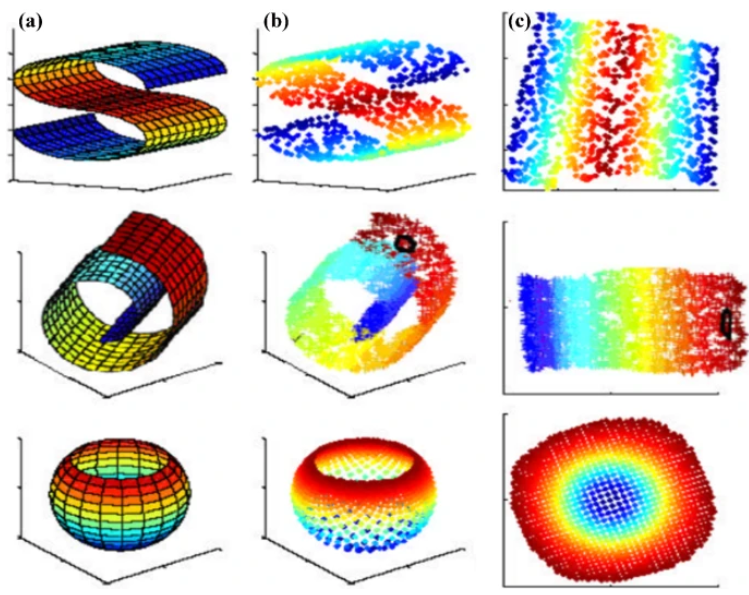
\includegraphics[width=0.5\textwidth]{figures/dim_reduction.png}\\
            \tiny{Source: \href{https://link.springer.com/article/10.1007/s40747-021-00637-x}{Link}}
      \end{center}
}

\begin{frame} 
      \frametitle{Introduction to Dimensionality Reduction}
      \textbf{Definition:} Dimensionality reduction is the process of reducing the number of features (variables) in a dataset while preserving as much important information as possible. It can be achieved by selecting a subset of original features or by transforming data to a new lower-dimensional space.\\
      \pause
      \smallskip
      \textbf{Motivation:} High-dimensional data can be challenging for both computation and analysis. Many machine learning algorithms suffer from the curse of dimensionality - increased features can lead to overfitting, higher computational cost, and difficulty in visualizing data. Reducing dimensionality can alleviate these issues by removing redundant features and noise.\\
      \pause 
      \smallskip
      \textbf{Benefits:} Fewer dimensions mean simpler models and faster computations, often improving learning performance and generalization. It also enables visualization of data in 2D or 3D, which is otherwise impossible for datasets with hundreds of features. For example, using PCA or t-SNE to project data down for visualization can reveal cluster structure in the data.
\end{frame}

\frame{
      \frametitle{Principal Component Analysis (PCA)}
      \begin{itemize}
            \item A linear dimensionality reduction technique that finds a new set of orthogonal axes (principal components) that capture the maximum variance in the data.
            \item In essence, PCA seeks the directions in the feature space along which the data varies the most, and uses those directions as new axes while discarding others with minimal loss of information.
            \item PCA identifies patterns in data by detecting correlations between original features. If variables are strongly correlated, PCA can replace them with a single principal component that represents their common information. 
      \end{itemize}
}

\frame{
      \frametitle{PCA: Algorithm} 
      \begin{itemize}
            \item \textbf{Standardize the data} - Ensure each feature has mean 0 (and optionally unit variance). This step is crucial if features have different units or scales.
            \item 
      \end{itemize}
}

% \frame{
%     \frametitle{Introduction to clustering}
%     \begin{itemize}
%         \item Clustering is a type of unsupervised learning, where the goal is to group similar objects together based on their features or attributes
%               \pause
%         \item We don't have any predefined labels or categories for the objects
%               \pause
%         \item The goal is to find natural groupings in the data
%               \pause
%         \item Can be used for a variety of applications, such as customer segmentation, image segmentation, anomaly detection, and recommendation systems
%               \pause
%         \item Clustering performance can be evaluated using metrics such as the within-cluster sum of squares (WCSS) and silhouette coefficient
%     \end{itemize}
% }

% \frame{
%     \frametitle{}
%     \begin{center}
%         {\Huge Dimensionality reduction}
%     \end{center}
% }

% \frame{
%     \frametitle{Dimensionality reduction}
%     \begin{itemize}
%         \item We have seen Latent Discriminant Analysis (LDA) in a previous lecture, today we will look at Principal Component Analysis (PCA)
%               \pause
%         \item Dimensionality reduction is a type of unsupervised learning, where the goal is to reduce the number of features in a dataset
%               \pause
%         \item The goal is to find a lower-dimensional representation of the data that preserves as much information as possible
%               \pause
%         \item Can be used for a variety of applications, such as data visualization, feature selection, and noise reduction
%               \pause
%         \item Dimensionality reduction performance can be evaluated using metrics such as the explained variance ratio
%     \end{itemize}
% }

% \frame{
%     \frametitle{}
%     \begin{center}
%         {\Huge Principal component analysis}
%     \end{center}
% }


% \frame{
%     \frametitle{Principal component analysis}
%     \begin{itemize}
%         \item Principal component analysis (PCA) is a dimensionality reduction technique that can be used to reduce the dimensionality of a dataset while preserving as much information as possible
%               \pause
%         \item PCA is a linear transformation that projects the data onto a lower-dimensional subspace
%               \pause
%         \item The principal components are the directions of maximum variance in the data
%               \pause
%         \item The first principal component is the direction of maximum variance, the second principal component is the direction of maximum variance that is orthogonal to the first principal component, and so on
%               \pause
%         \item The explained variance ratio is the ratio of the variance of a principal component to the total variance
%               \pause
%         \item The explained variance ratio can be used to determine the number of principal components to keep
%     \end{itemize}
% }

% \frame{
%     \frametitle{Eigenvalues and Eigenvectors:}
%     \begin{itemize}
%         \item Eigenvalues represent the amount of variance captured by each principal component. Higher eigenvalues correspond to more important principal components.
%         \item Eigenvectors are the directions of the axes along which the data varies the most. Each eigenvector is associated with a specific eigenvalue. These eigenvectors form the principal components.
%     \end{itemize}
% }

% \frame{
%     \frametitle{}
%     \begin{center}
%         {\Huge K-means clustering}
%     \end{center}
% }

% \frame{
%     \frametitle{K-means clustering}
%     \begin{itemize}
%         \item K-means clustering is an iterative clustering algorithm that can be used to find natural groupings in a dataset
%               \pause
%         \item The algorithm starts by randomly assigning each observation to a cluster
%               \pause
%         \item The algorithm then iteratively updates the cluster centers and assigns each observation to the nearest cluster center
%               \pause
%         \item The algorithm stops when the cluster assignments no longer change
%               \pause
%         \item The within-cluster sum of squares (WCSS) is the sum of the squared distances between each observation and its cluster center
%               \pause
%         \item The silhouette coefficient is a measure of how well an observation is clustered
%               \pause
%         \item The silhouette coefficient ranges from -1 to 1, where a value close to 1 indicates that the observation is well clustered
%     \end{itemize}
% }

\end{document}